\chapter{Analyse}

\begin{itemize}
  \item Daten
  \begin{itemize}
    \item Welche Listen wurden verwendet?
    \item Woher kommen die?
  \end{itemize}
  \item Statistische Auswertung
  \begin{itemize}
    \item Gesamtauswetungen
    \item Kleine Abschnitte für Einzelauswertungen der Tests
  \end{itemize}
  \item Disskusion
  \item Bewertung
\end{itemize}
\todo{Samuel}


\begin{figure}[H]
  \centering
  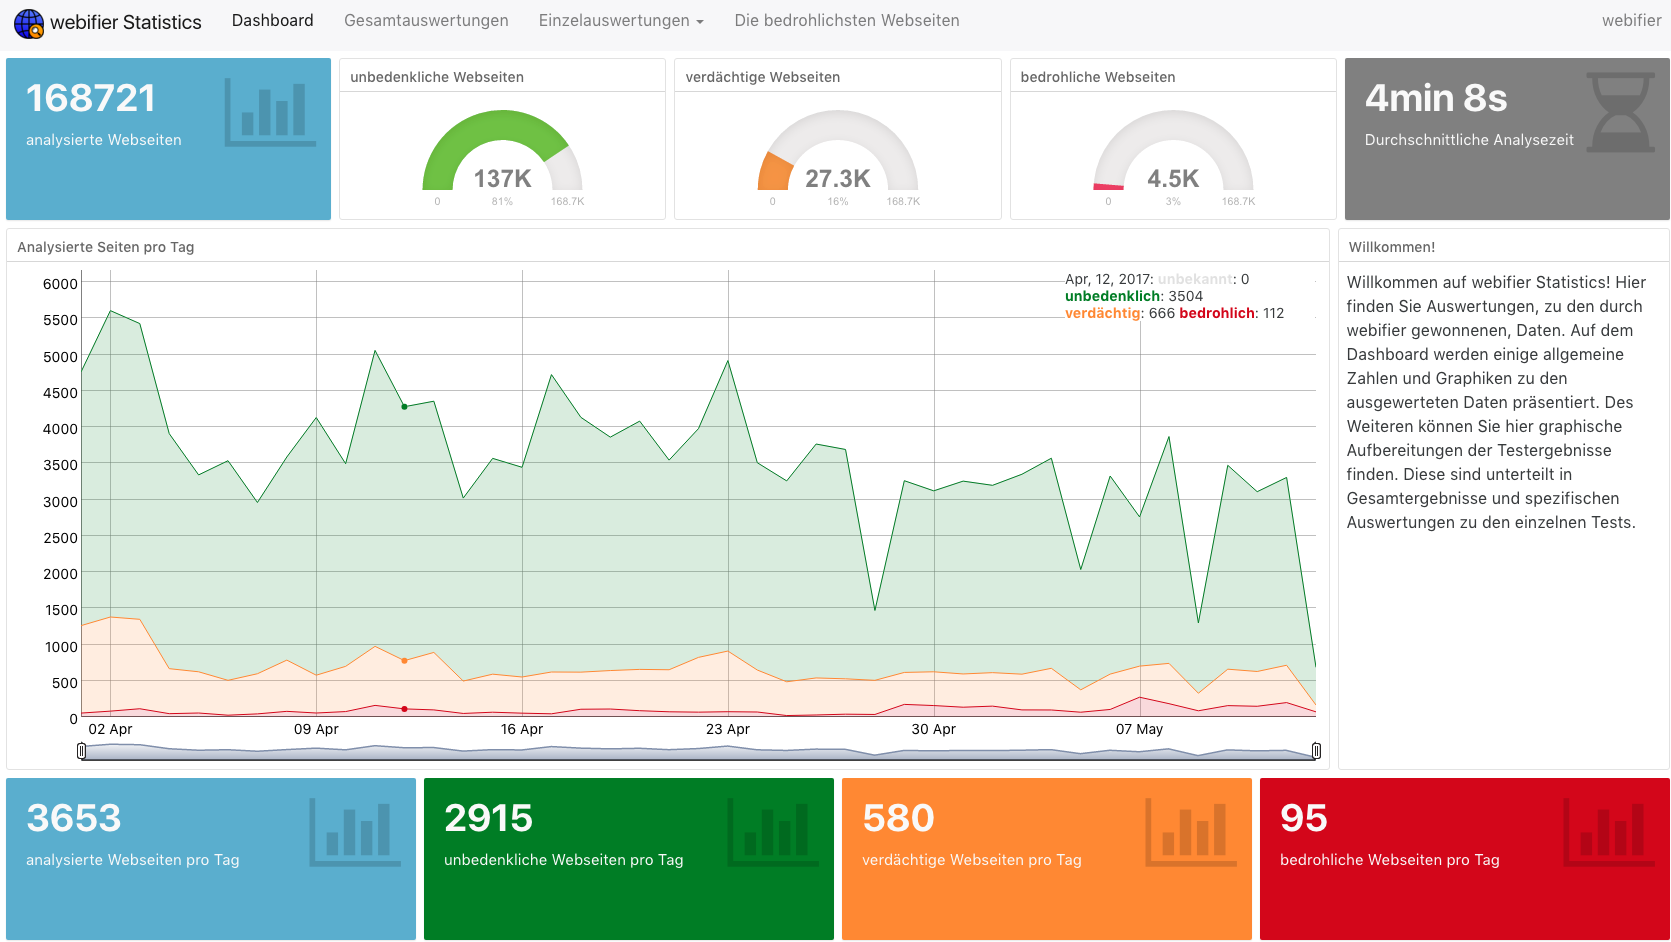
\includegraphics[width=15cm]{images/stats/dashboard}
  \caption{Webifier Statistics Dashboard}
  \label{fig:dashboard}
\end{figure}


\section{Gesamtauswertungen}

\todo{Jani}

\begin{figure}[H]
  \centering
  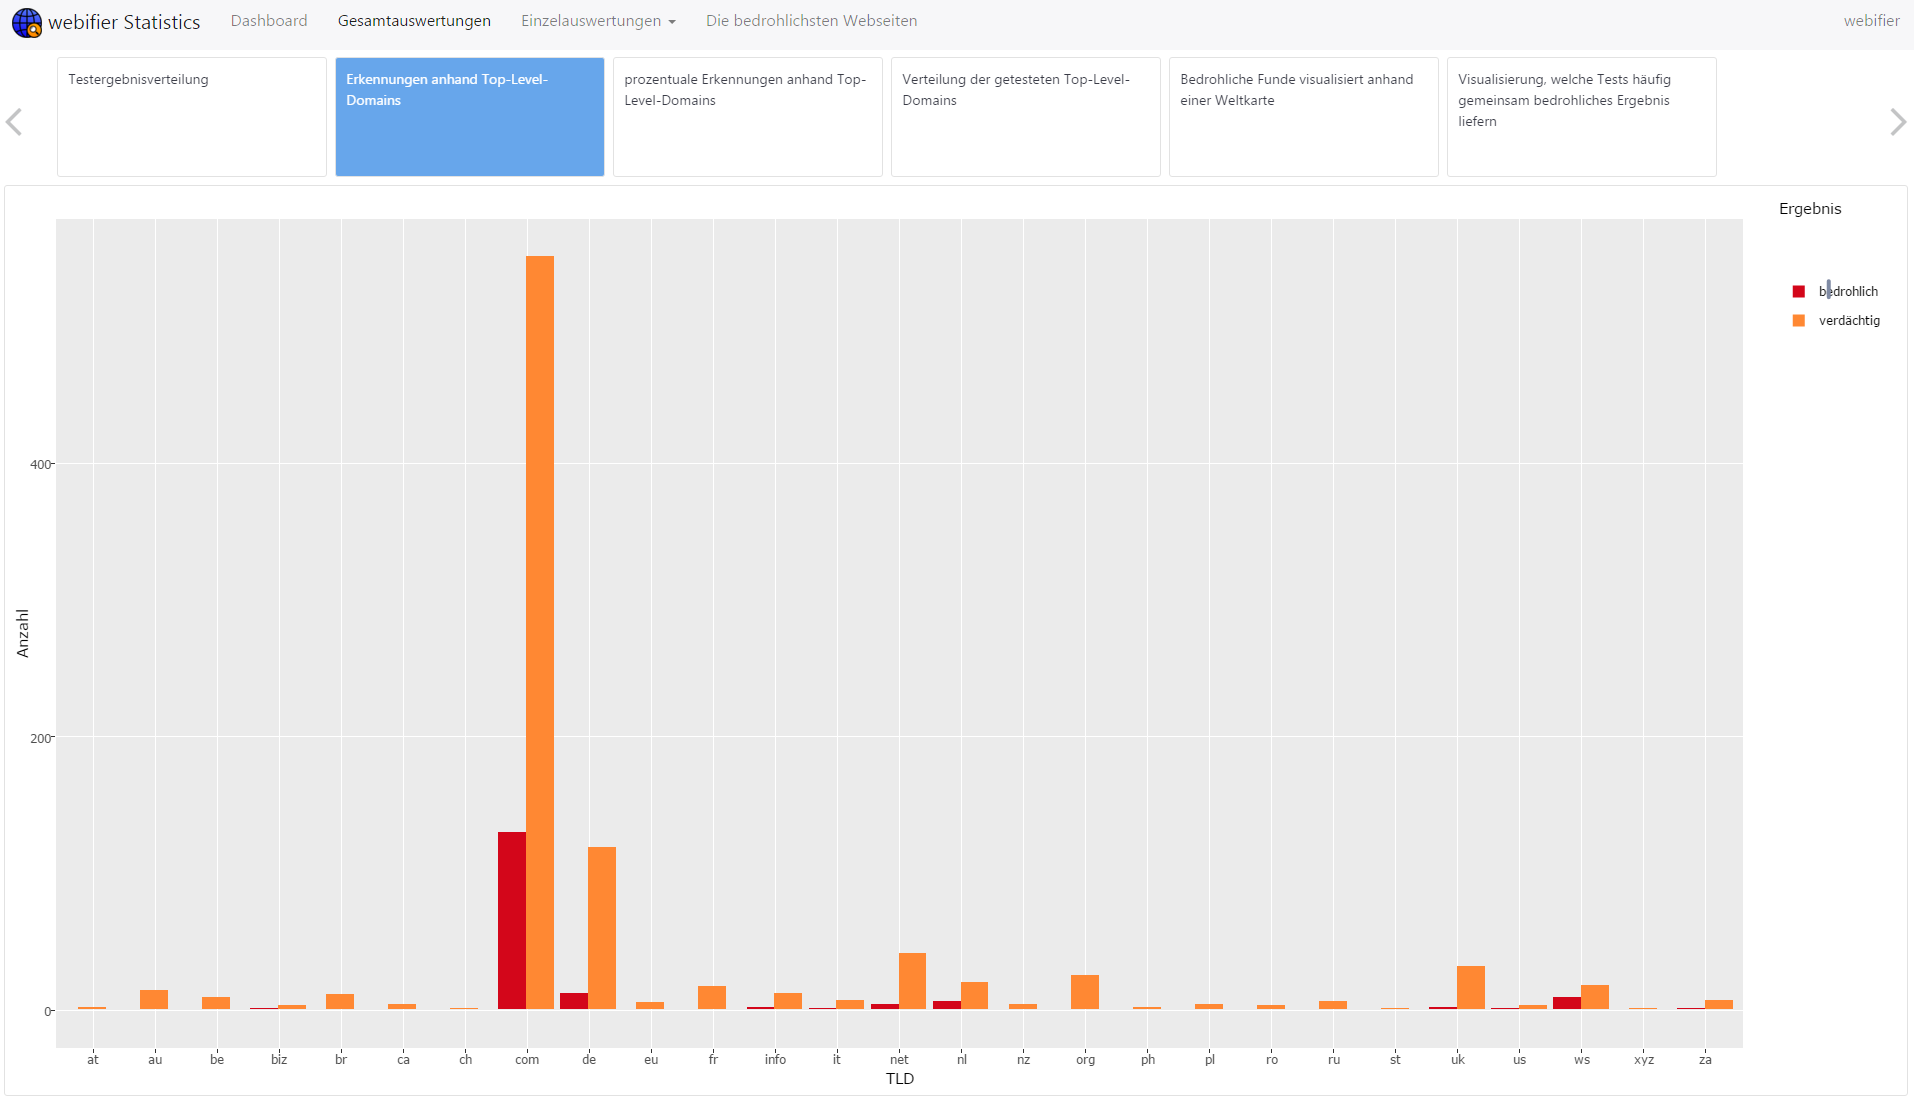
\includegraphics[width=15cm]{images/stats/tlderkennungen}
  \caption{Erkennungen anhand Top-Level-Domains}
  \label{fig:tlderkennungen}
\end{figure}


\begin{figure}[H]
  \centering
  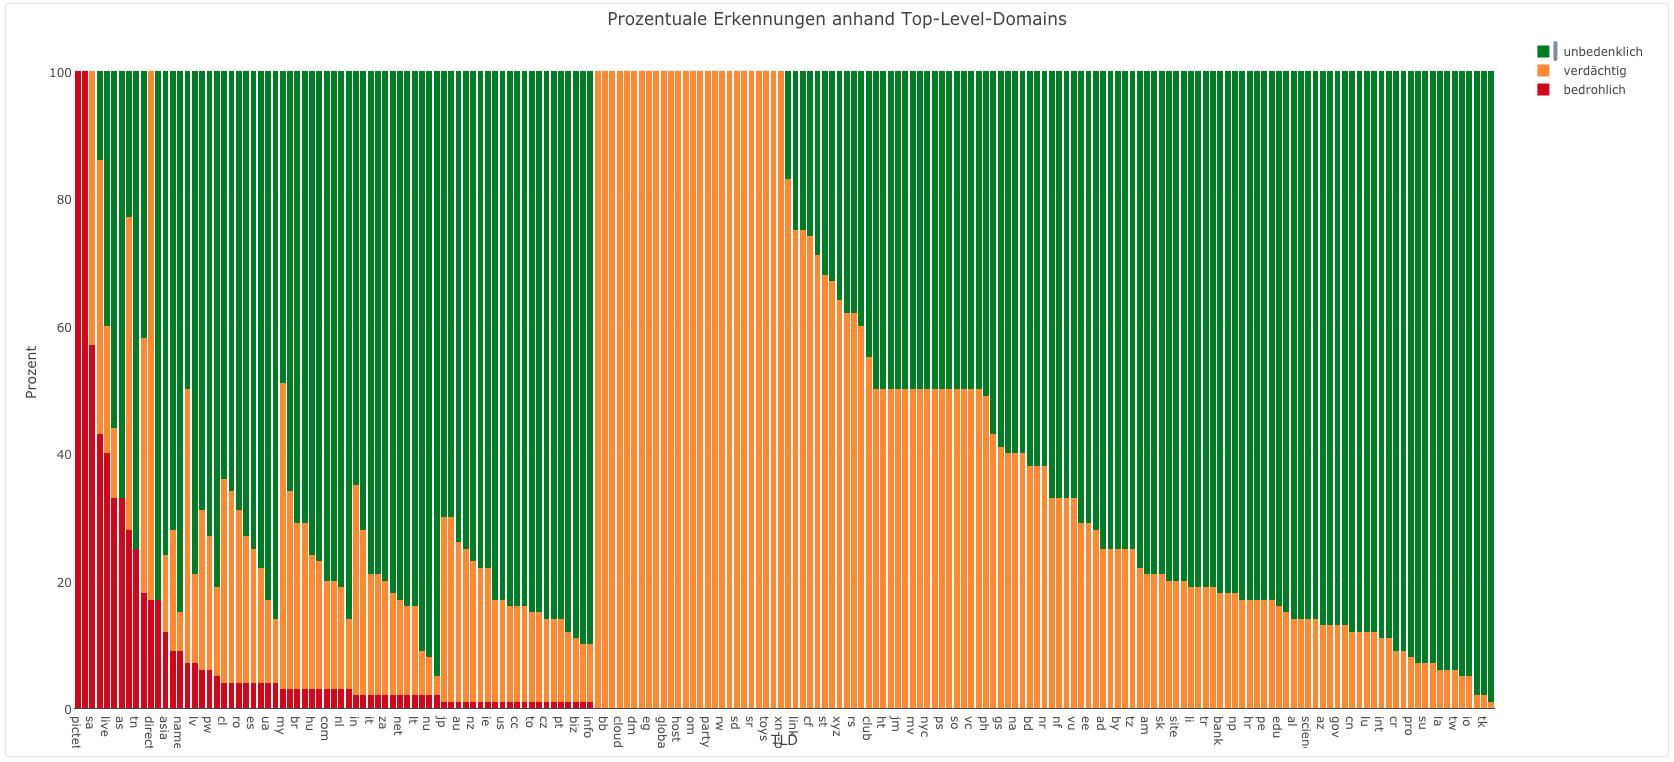
\includegraphics[width=15cm]{images/stats/tldprozentual}
  \caption{prozentuale Erkennungen anhand Top-Level-Domains}
  \label{fig:tldprozentual}
\end{figure}


\begin{figure}[H]
  \centering
  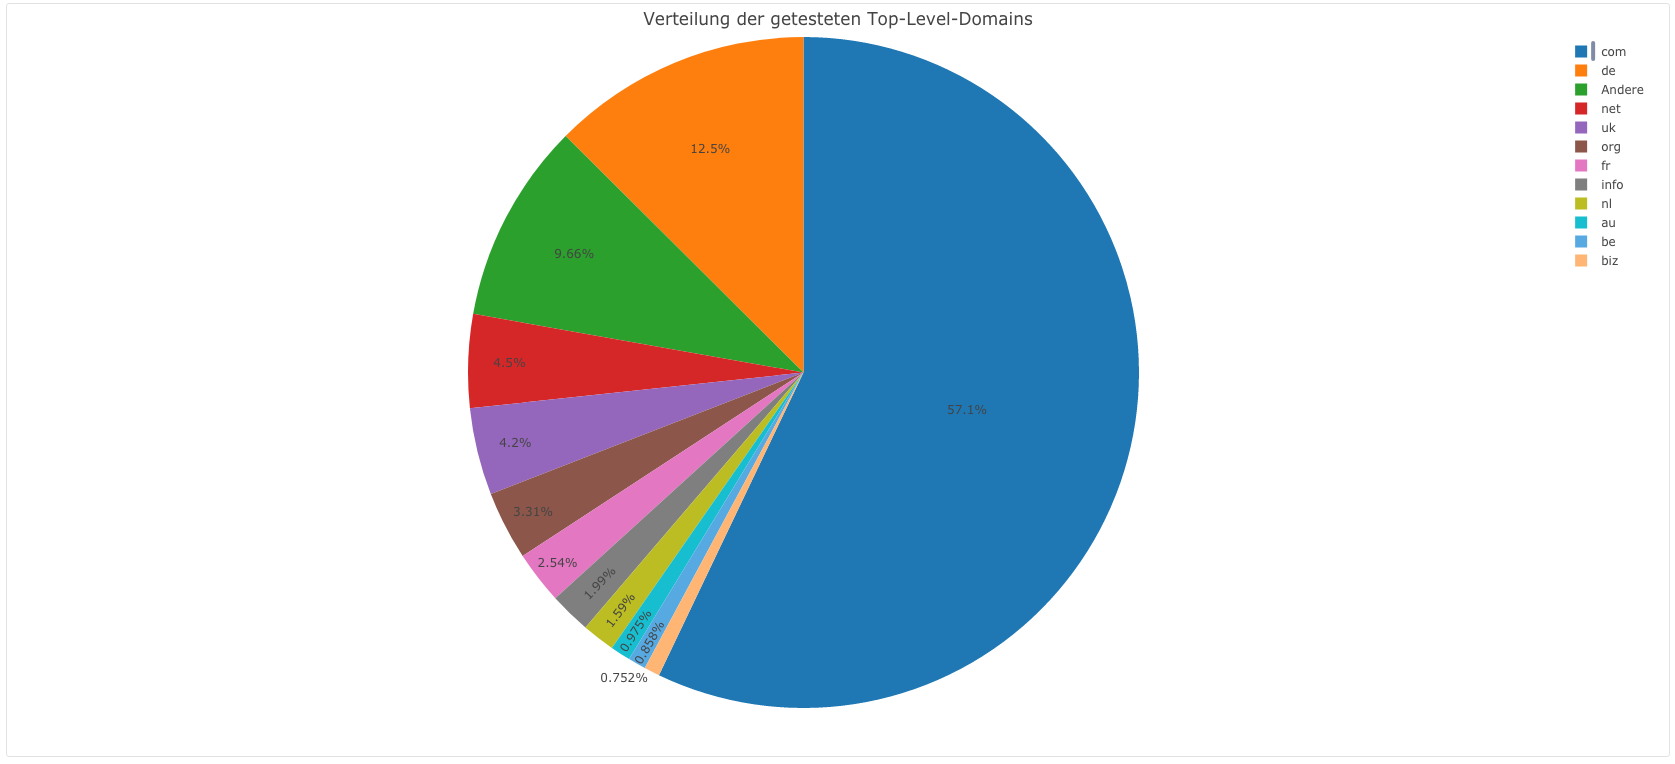
\includegraphics[width=15cm]{images/stats/tldverteilung}
  \caption{Verteilung der getesteten Top-Level-Domains}
  \label{fig:tldverteilung}
\end{figure}


\begin{figure}[H]
  \centering
  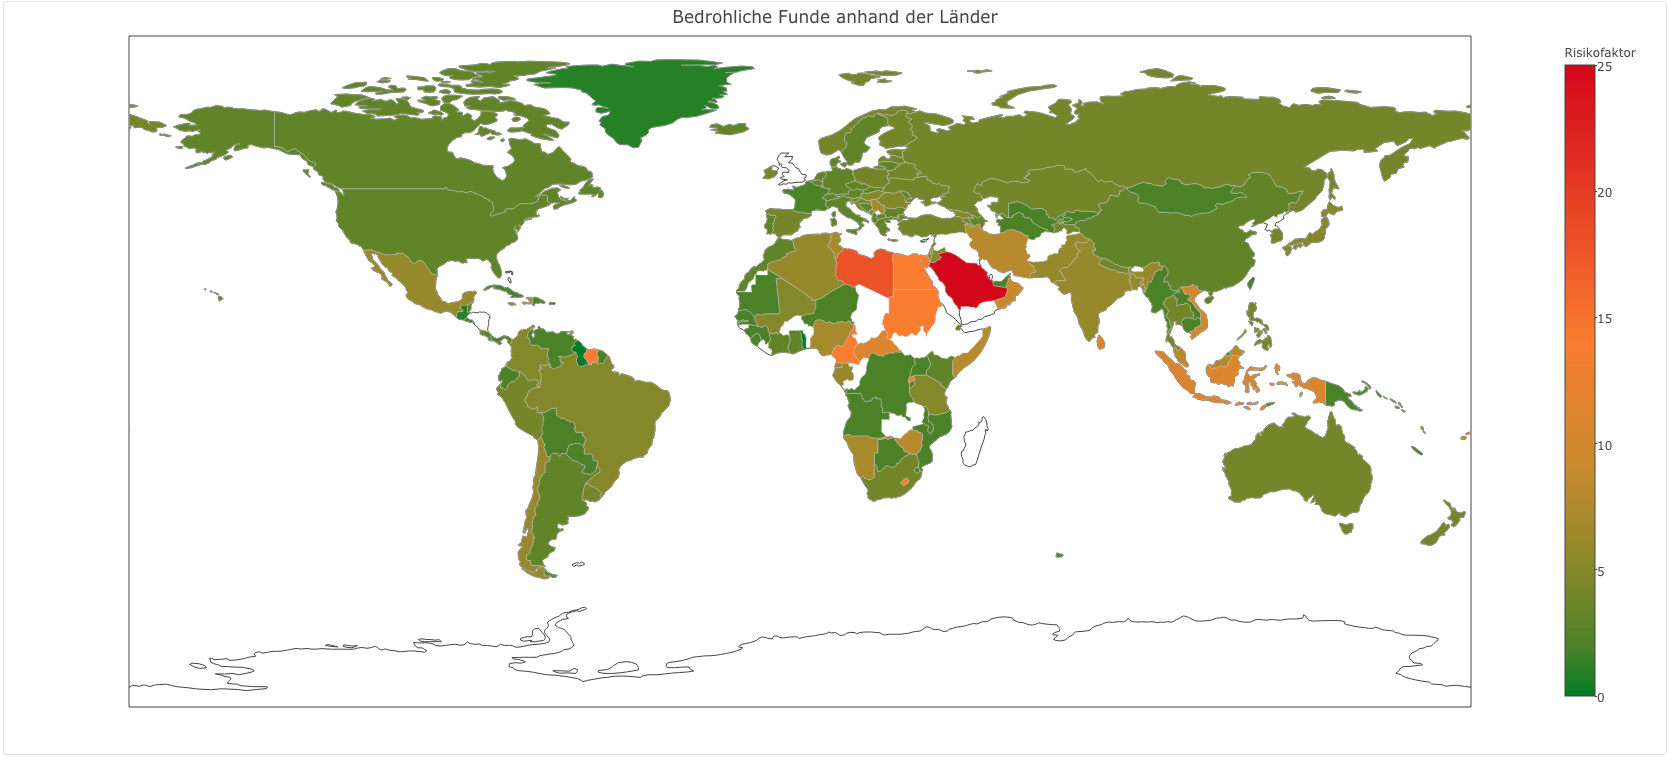
\includegraphics[width=15cm]{images/stats/weltkarte}
  \caption{Bedrohliche Funde visualisiert anhand einer Weltkarte}
  \label{fig:weltkarte}
\end{figure}


\begin{figure}[H]
  \centering
  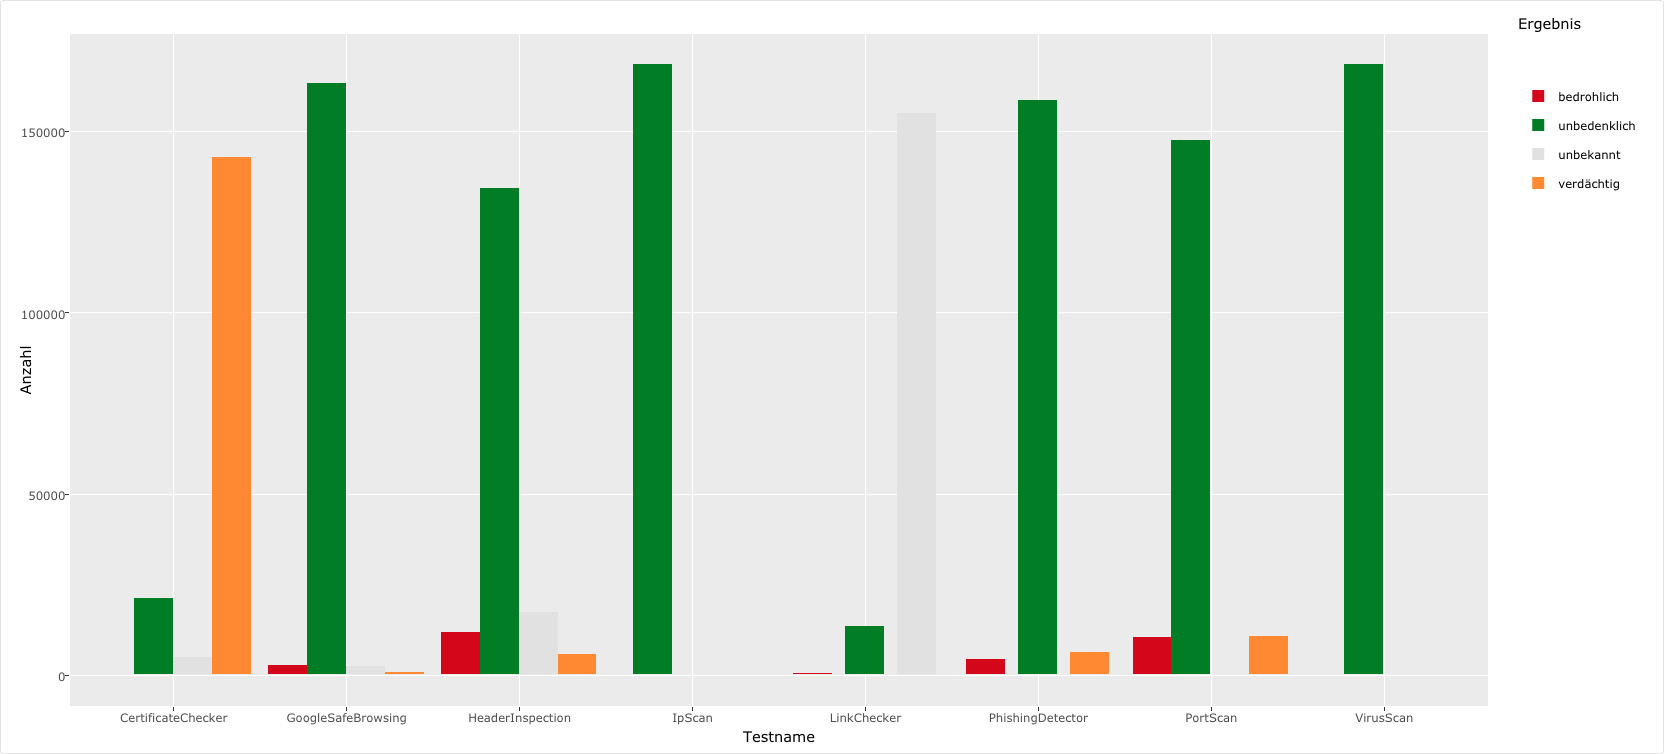
\includegraphics[width=15cm]{images/stats/ergebnisverteilung}
  \caption{Testergebnisverteilung}
  \label{fig:ergebnisverteilung}
\end{figure}


\begin{figure}[H]
  \centering
  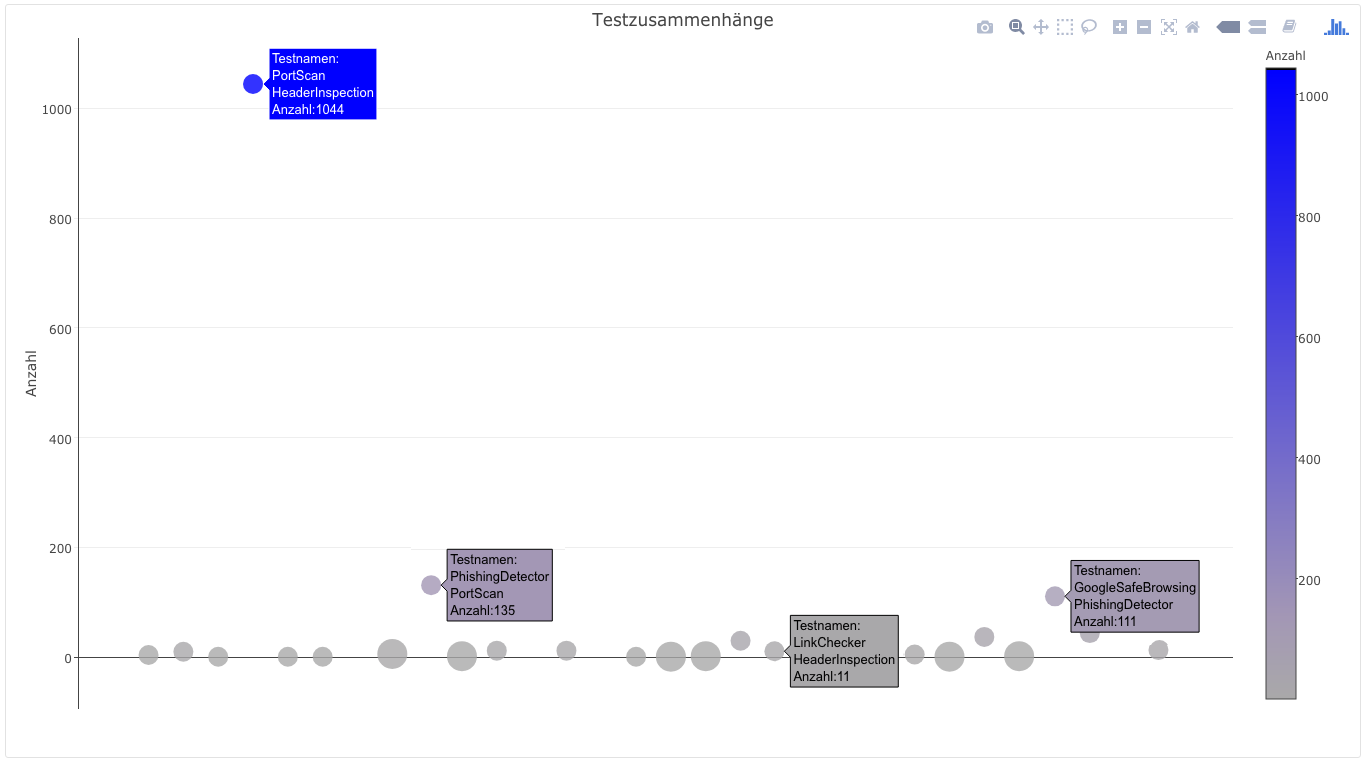
\includegraphics[width=15cm]{images/stats/testzusammenhaenge}
  \caption{Visualisierung der Testzusammenhänge}
  \label{fig:testzusammenhaenge}
\end{figure}


\begin{figure}[H]
  \centering
  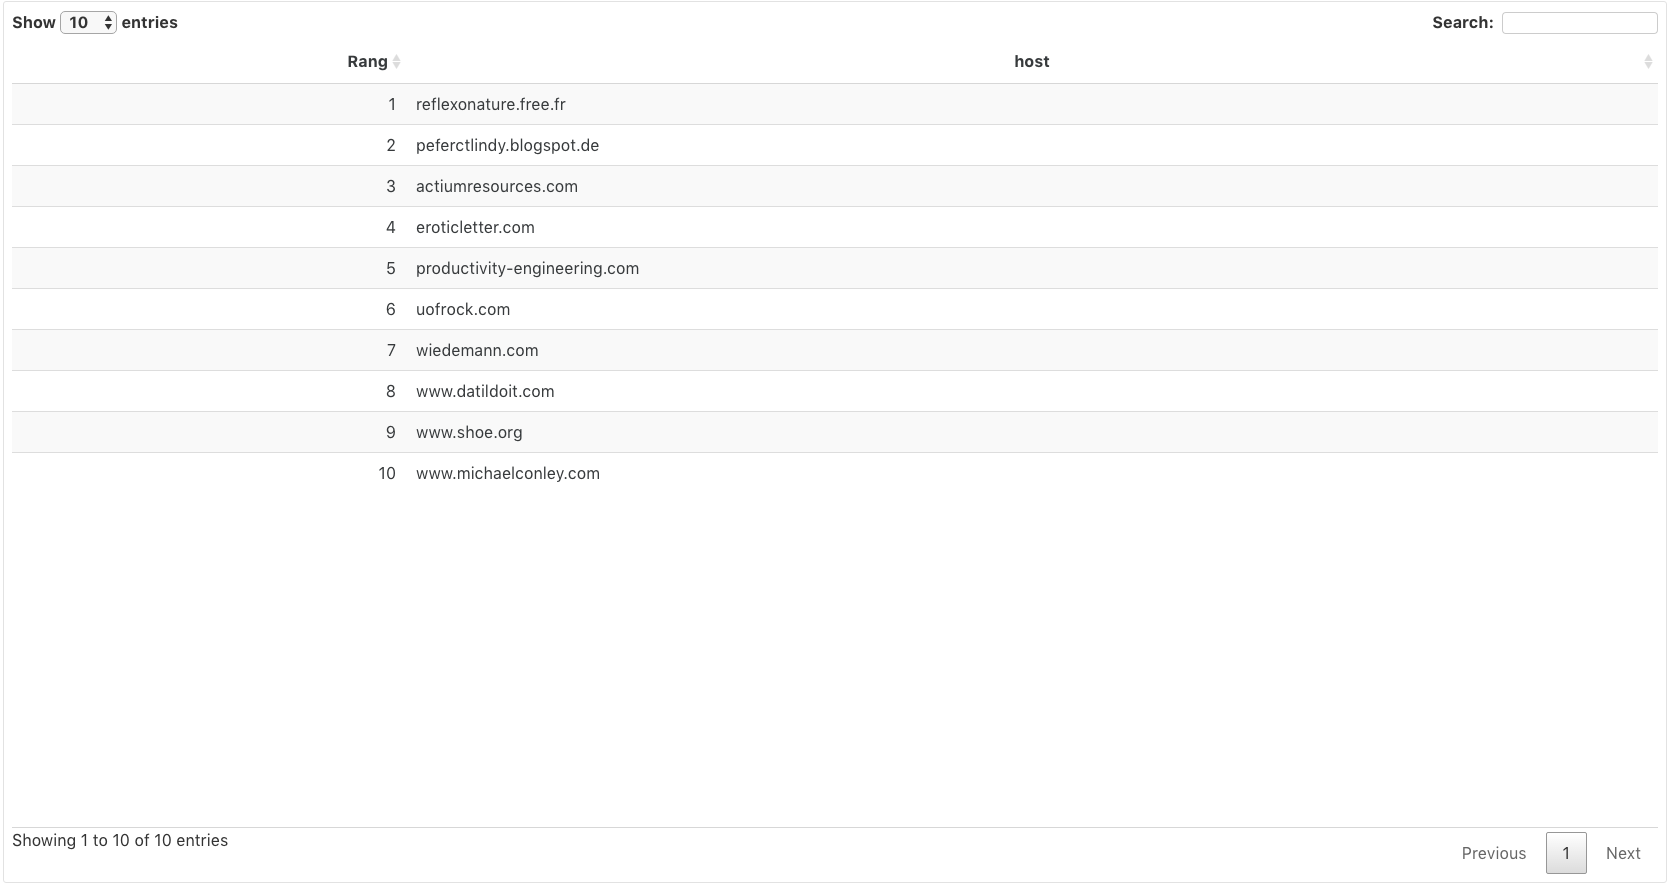
\includegraphics[width=15cm]{images/stats/top10}
  \caption{Top 10: Die bedrohlichsten Webseiten}
  \label{fig:top10}
\end{figure}


\section{Einzelauswertungen}
\begin{figure}[H]
  \centering
  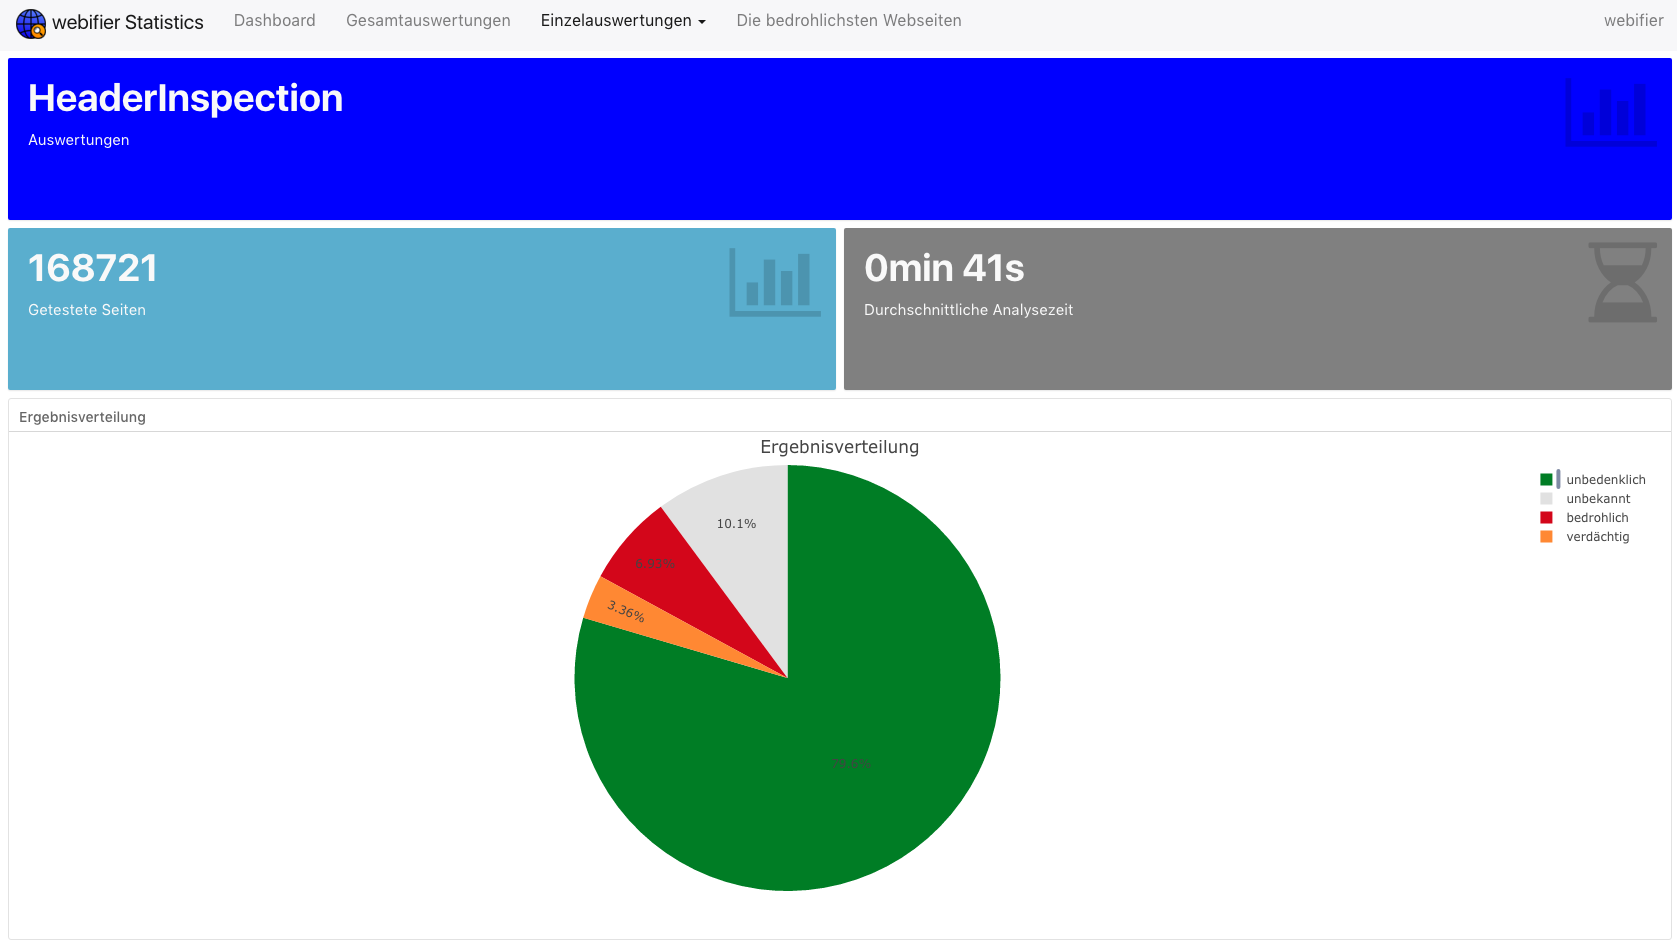
\includegraphics[width=15cm]{images/stats/headerinspection}
  \caption{Einzelauswertung: Vergleich in verschiedenen Browsern}
  \label{fig:headerinspection}
\end{figure}


\begin{figure}[H]
  \centering
  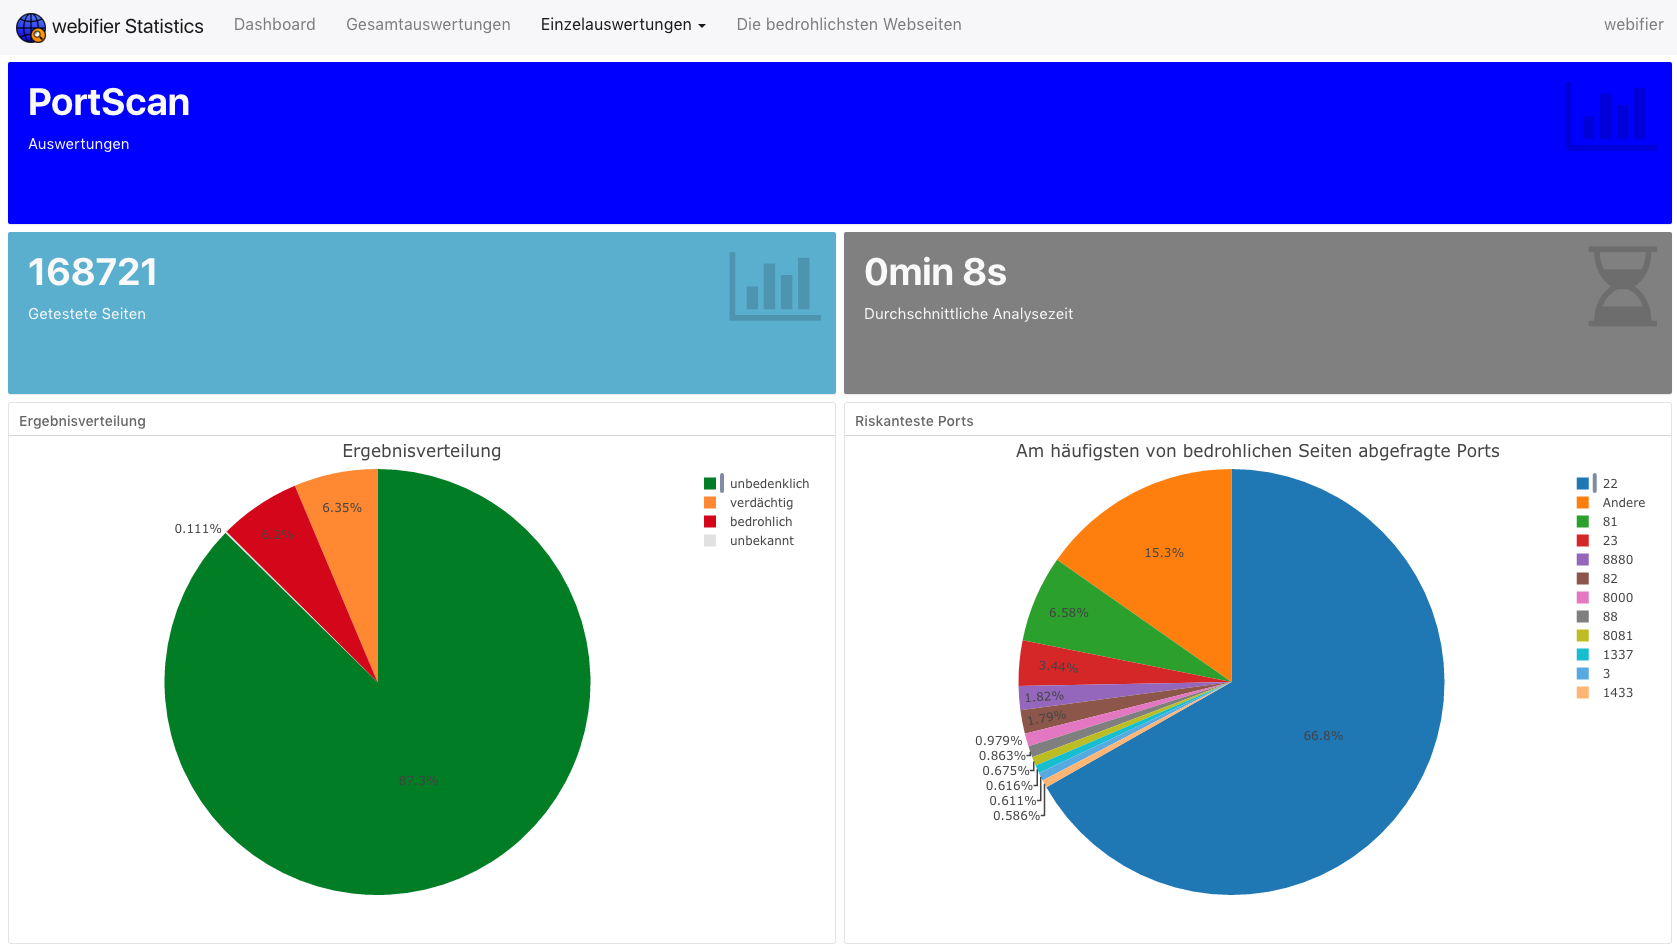
\includegraphics[width=15cm]{images/stats/portscan}
  \caption{Einzelauswertung: Überprüfung der Port-Nutzung}
  \label{fig:virenscan}
\end{figure}


\begin{figure}[H]
  \centering
  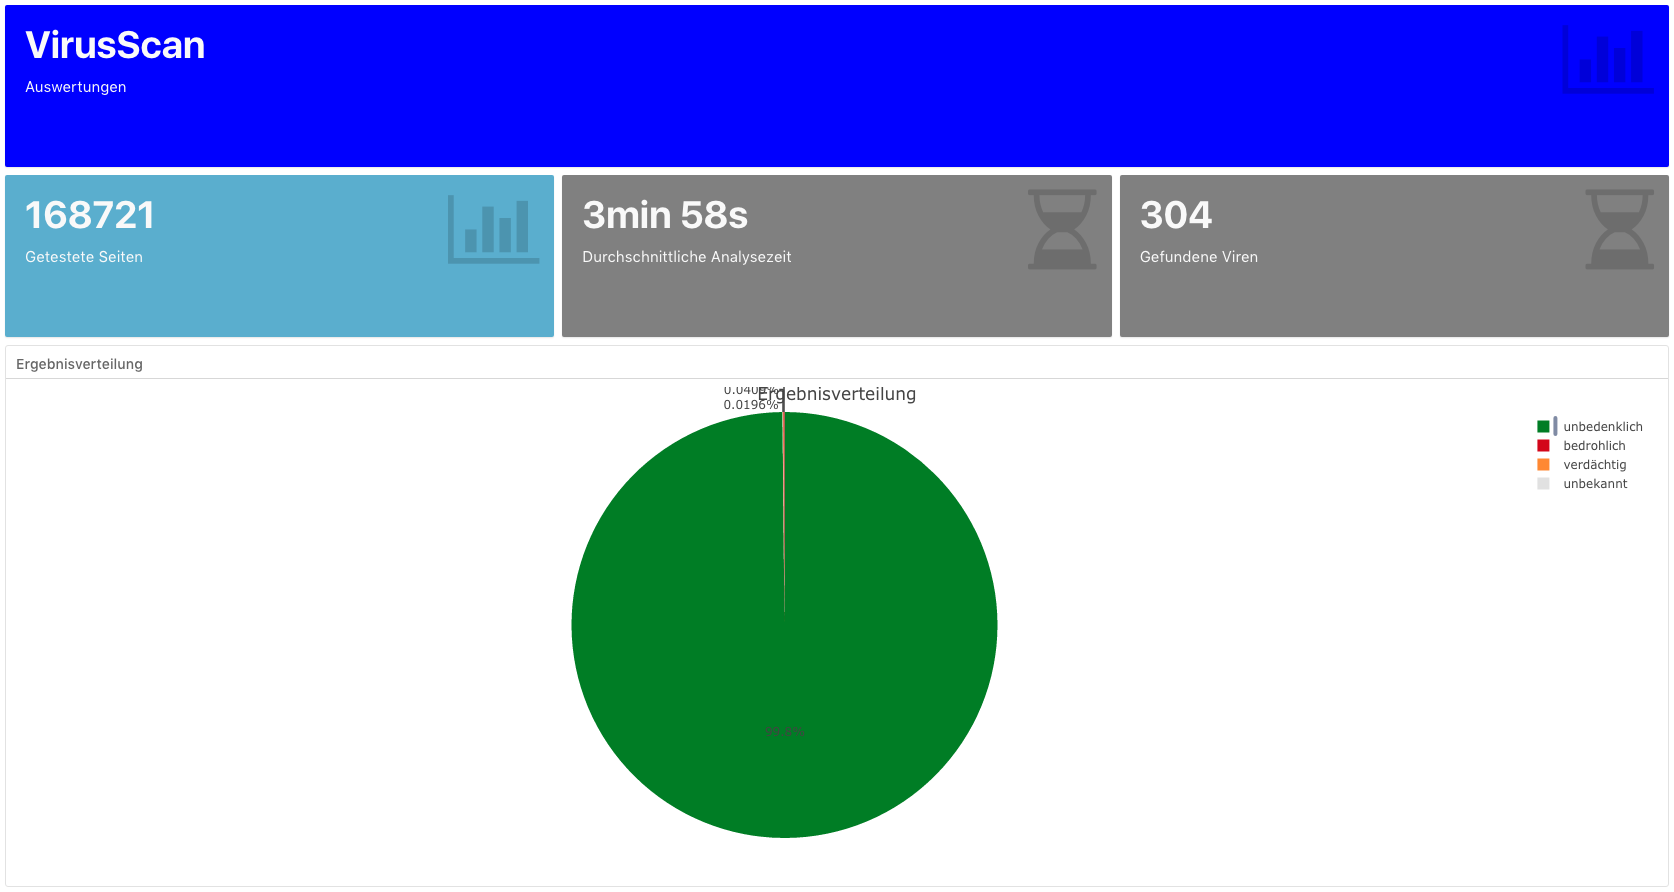
\includegraphics[width=15cm]{images/stats/virusscan}
  \caption{Einzelauswertung: Virenscan der Webseite}
  \label{fig:virusscan}
\end{figure}

\todo{Jani}


\subsection{Virenscan der Webseite}
\begin{figure}[H]
  \centering
  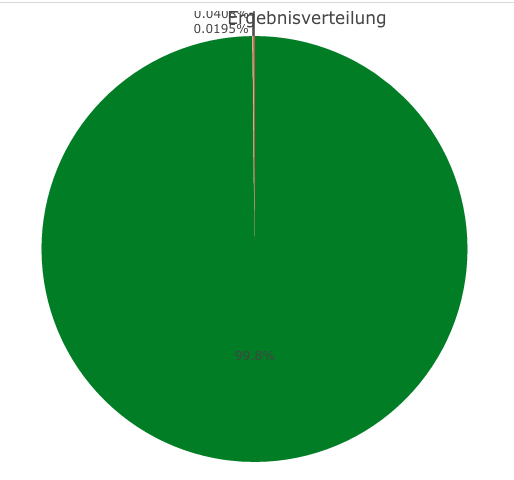
\includegraphics[width=5cm]{images/stats/diavirenscan}
  \caption{Virenscan der Webseite - Testergebnisverteilung}
  \label{fig:diavirenscan}
\end{figure}
\todo{Samuel}

\subsection{Vergleich in verschiedenen Browsern}
\begin{figure}[H]
  \centering
  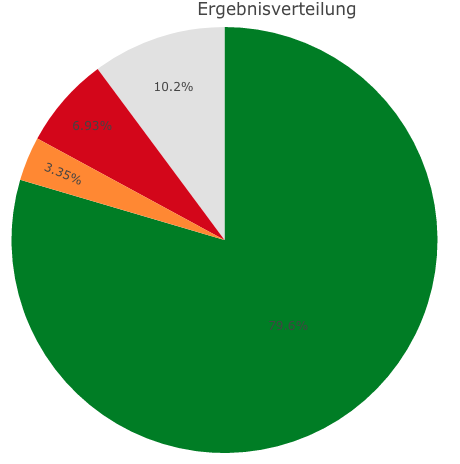
\includegraphics[width=5cm]{images/stats/diaheaderinspection}
  \caption{Vergleich in verschiedenen Browsern - Testergebnisverteilung}
  \label{fig:diaheaderinspection}
\end{figure}
\todo{Daniel}

\subsection{Überprüfung der Port-Nutzung}
\begin{figure}[H]
  \centering
  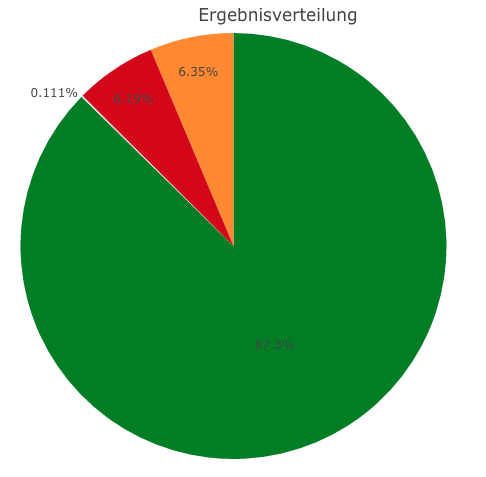
\includegraphics[width=5cm]{images/stats/diaportscan}
  \caption{Überprüfung der Port-Nutzung - Testergebnisverteilung}
  \label{fig:diaportscan}
\end{figure}
\todo{Jani}

\subsection{Überprüfung der IP-Nutzung}
\begin{figure}[H]
  \centering
  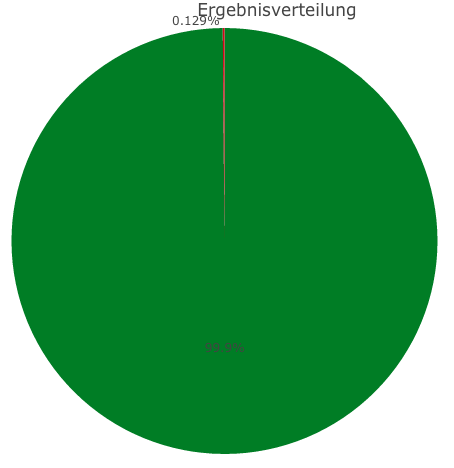
\includegraphics[width=5cm]{images/stats/diaipscan}
  \caption{Überprüfung der IP-Nutzung - Testergebnisverteilung}
  \label{fig:diaipscan}
\end{figure}
\todo{Jani}

\subsection{Prüfung aller verlinkten Seiten}
\begin{figure}[H]
  \centering
  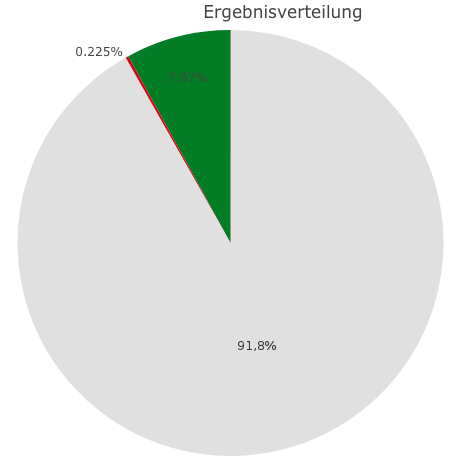
\includegraphics[width=5cm]{images/stats/dialinkchecker}
  \caption{Prüfung aller verlinkten Seiten - Testergebnisverteilung}
  \label{fig:dialinkchecker}
\end{figure}
\todo{Samuel}

\subsection{Google Safe Browsing}
\begin{figure}[H]
  \centering
  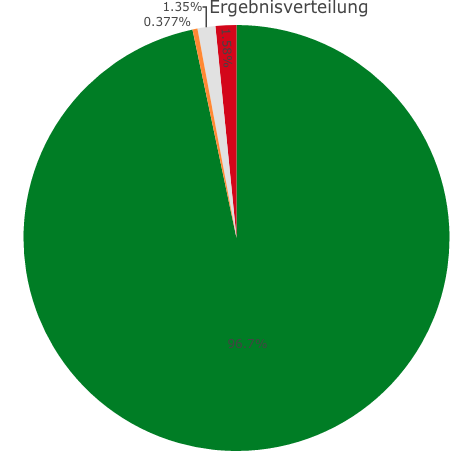
\includegraphics[width=5cm]{images/stats/diagoogle}
  \caption{Google Safe Browsing - Testergebnisverteilung}
  \label{fig:diagoogle}
\end{figure}
\todo{Daniel}

\subsection{Überprüfung des SSL-Zertifikats}
\begin{figure}[H]
  \centering
  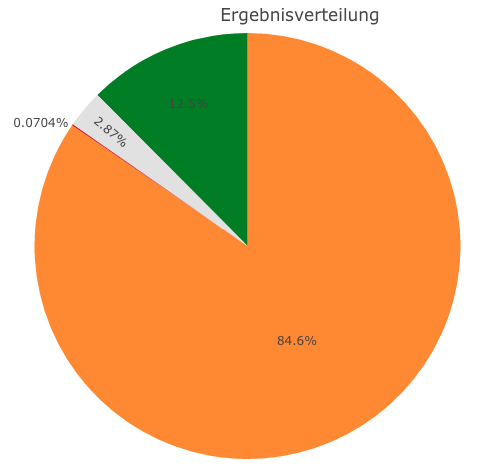
\includegraphics[width=5cm]{images/stats/diacertificate}
  \caption{Überprüfung des SSL-Zertifikats - Testergebnisverteilung}
  \label{fig:diacertificate}
\end{figure}
\todo{Samuel}

\subsection{Erkennung von Phishing}
\begin{figure}[H]
  \centering
  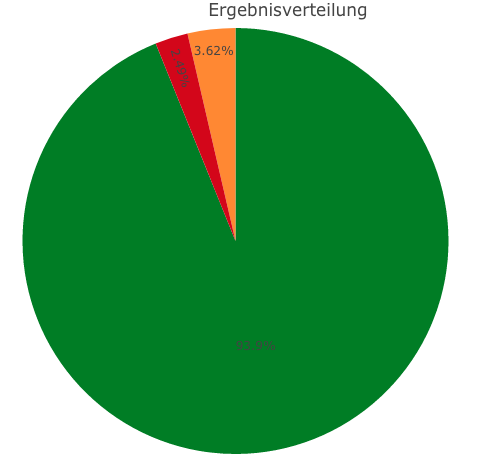
\includegraphics[width=5cm]{images/stats/diaphishing}
  \caption{Erkennung von Phishing - Testergebnisverteilung}
  \label{fig:diaphishing}
\end{figure}
\todo{Samuel}

\section{Bewertung der Ergebnisse}
